% File hicss51.tex
%%
%% Based on the style files for ACL 2015 by 
%% car@ir.hit.edu.cn, gdzhou@suda.edu.cn


\documentclass[10pt]{article}
\usepackage[letterpaper]{geometry}
\usepackage{hicss51}
\usepackage{times}
\usepackage[none]{hyphenat}
\usepackage{url}
\usepackage{latexsym}
%\usepackage{minted}
\usepackage{indentfirst}
\usepackage{graphicx}
%\graphicspath{{images/}}
\usepackage{wrapfig}
\usepackage{todonotes}
\usepackage{hyperref}
\usepackage[utf8]{inputenc}
\newcommand{\sansserifformat}[1]{\fontfamily{cmss}{ #1}}%

%\setlength\titlebox{5cm}


% You can expand the titlebox if you need extra space
% to show all the authors. Please do not make the title box
% smaller than 5cm (the original size).

\usepackage{booktabs}

\title{Open Source Intelligence - Development of a Trend Radar utilizing a Systematic Literature Review}

\author{Franz Kayser \\
  ESG \\
  {\underline{ franz.kayser@esg.de}} \\\And
  Thomas Mayer \\
  ESG  \\
  {\underline{ thomas3.mayer@esg.de} }\\\And 
  Michael Bücker \\
  FH Münster -- University of Applied Sciences\\
  {\underline{michael.buecker@fh-muenster.de}} \\}

\date{}

\begin{document}
\maketitle
\begin{abstract}
    Open Source Intelligence (OSINT) is experiencing an intensive discourse,
    heightened since the Russian invasion of Ukraine. However, despite numerous attempts
    at standardized definitions, the intelligence discipline remains ambiguous. This paper
    introduces a practice-validated OSINT trend radar, categorizing technologies by maturity,
    intelligence cycle phase, and use case. Serving as a profound knowledge base and tool for
    identifying research gaps, the radar emerges from a structured design process. Sixty
    studies underwent categorization and validation through expert interviews,
    revealing the absence of a autonomous third-generation OSINT
    system in Germany. Technological gaps, in the planning and direction and
    dissemination and integration phases, are evident. Although intelligent support
    technologies were identified, practical implementation lags behind theory. The human
    factor remains central to the OSINT process. Future research should develop
    applications for underserved phases and examine why proven applications aren't widely
    adopted, focusing on legal, ethical, political, and social factors.
\end{abstract}

\section{Introduction} \label{sec:introduction}

OSINT, the process of gathering intelligence from public data, has gained considerable attention, particularly since
the 2022 Russian invasion of Ukraine \cite{DosPassos.2017}. Real-time analysis of social media has proven pivotal in revealing
valuable insights \cite{SmithBoyle.24.07.2023}. Despite numerous attempts to define OSINT
\cite{Hwang.2022, PastorGalindo.2020, Yogish.2021}, controversy persists, influenced by ongoing advancements in computer and
data sciences that continuously enhance collection and analysis capabilities \cite{Ghioni.2023, Williams.2018}.
The surge in open communication channels has led to an "information explosion" \cite{DosPassos.2017, Hwang.2022, Yogish.2021},
making previously restricted data publicly accessible \cite{Hwang.2022, Williams.2018}, reshaping intelligence paradigms \cite{Dokman.2020}.
Despite the heightened interest, fundamental scientific literature in the field remains limited \cite{HerreraCubides.2020},
failing to keep pace with rapid developments \cite{Ghioni.2023, Williams.2018}. Key questions regarding the existence of
autonomous third-generation OSINT systems \cite{PastorGalindo.2019, PastorGalindo.2020} remain unanswered
\cite{Ghioni.2023, PastorGalindo.2020, Yogish.2021} and significant OSINT use cases unexplored
\cite{AlKilani.2021, Dokman.2020, Ghioni.2023}, lacking qualitative field research to bridge theoretical concepts with
practical implementation \cite{HerreraCubides.2020, PastorGalindo.2019}. This study thus addresses the research question:
question: \textit{How can current OSINT trends, in the form of technologies and their characteristics, particularly maturity levels and use cases, be presented in a trend radar and validated by security sector experts?}


This paper investigates current OSINT trends, adopting the Design Science Research Model (DSRM) \cite{Peffers.2007}.
The methodology involves a systematic literature review \cite{Webster.2002} to analyze and classify relevant OSINT literature.
Subsequently, OSINT technologies and their characteristics will be visualized in a trend radar, validated through systematizing
interviews with security sector experts \cite{Bogner.2014}, and evaluated using qualitative content analysis \cite{Billings.1997}.


\section{Theoretical Background} \label{sec:theoreticalbackground}

The domain of OSINT is continuously expanding due to the ongoing improvements of
collecting and analysis possibilities \cite{Ghioni.2023, Williams.2018}. In
addition, the new means and methods of communication associated with advances in information
and communication technology have turned OSINT into a complex discipline
\cite{Benes.2013, Williams.2018}.

\subsection{Open Source Intelligence (OSINT) and its Components}

One of the earliest and still frequently referenced definitions \cite{DosPassos.2017}
was published by \cite{NorthAtlanticTreatyOrganization.2001} in 2001: \textit{"OSINT is information that has been
    deliberately discovered, discriminated, distilled, and disseminated to a selected audience,
    [...], in order to address a specific question. OSINT, [...] thus applies the proven
    process of intelligence to the broad diversity of open sources [...] and creates
    intelligence."} However, today the discipline is no longer seen as a purely governmental
matter. Private research institutions and organizations \cite{Bohm.2021,Mercado.2005} are
also massively driving the development of such systems
\cite{Dokman.2020, Ghioni.2023}. The focus is thereby shifting to
developing OSINT into a robust, autonomous solution (referred to as third-generation) \cite{PastorGalindo.2019}.

\subsection{Intelligence and Intelligence Cycle}

The core task of OSINT is to generate intelligence
as a basis for decision-making
\cite{Breakspear.2013,NorthAtlanticTreatyOrganization.2001}. The generation process of such an intelligence product
is referred to as intelligence cycle \cite{CentralIntelligenceAgency.1987}.
It represents the central element of every intelligence discipline \cite{Reuser.2017}. 
The link between the phases is that the result of each preceding phase serves as input for the subsequent phase \cite{JointChiefsofStaffU.S.Army.2013}, continuously iterated to meet new requirements and demands \cite{Gibson.2016}.
Today, to represent external influences or the
assignment of responsibilities \cite{Lowenthal.2020,Phythian.2013}, numerous
variations can be found \cite{Reuser.2017}. The
Intelligence Cycle should hence be seen less as a guideline and more as an informal
coordination element \cite{Hwang.2022}.
In 2013, \cite{JointChiefsofStaffU.S.Army.2013} segmented the cycle into 6 phases  (see figure \ref{fig: intelligence cycle}).

\begin{figure}[h]
    \centering
    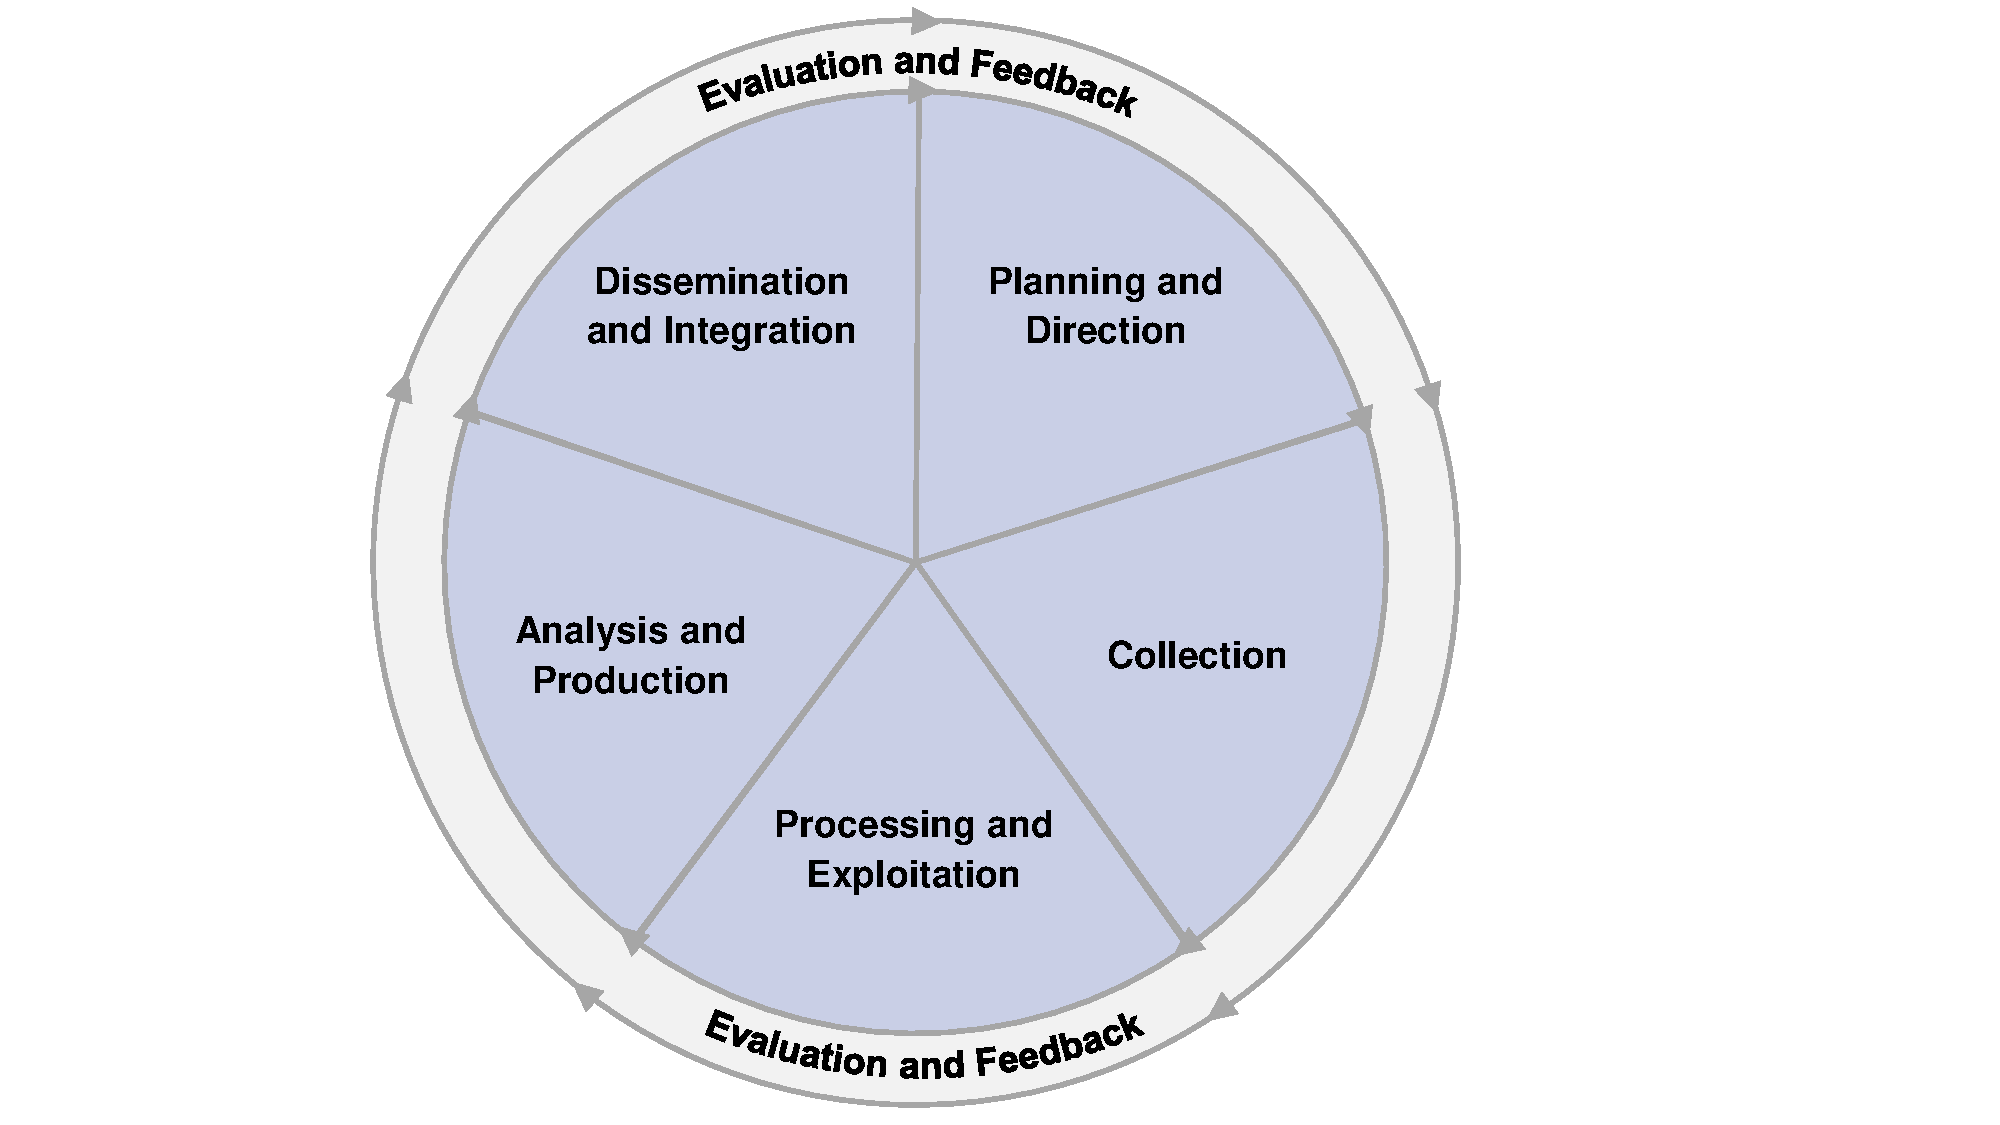
\includegraphics[clip,width=0.8\linewidth]{PDF/images/crop_Intelligence Cycle}
    \caption{Intelligence Cycle, according to \cite{JointChiefsofStaffU.S.Army.2013}}
    \label{fig: intelligence cycle}
\end{figure}

The planning and direction phase combines the identification, definition, prioritization and monitoring
of the requirements \cite{JointChiefsofStaffU.S.Army.2013}.
The collection phase refers to the gathering of raw data \cite{CentralIntelligenceAgency.1987}.
It consists of iterative repetition of research
\cite{NorthAtlanticTreatyOrganization.2001} to make the query more precise with each run
\cite{PastorGalindo.2020}. The processing and utilization phase involves condensing
these data volumes into action-relevant information
\cite{JointChiefsofStaffU.S.Army.2013}.
Analysis and production refers to the synthesis of the information obtained into a timely and accurate intelligence product
\cite{Hwang.2022, NorthAtlanticTreatyOrganization.2001}.
The final phase consists of handing over the product to the "customer" in a
usable form \cite{CentralIntelligenceAgency.2023, Williams.2018}.
Evaluation and feedback are not to be regarded as individual phases
but take place continuously, to achieve progressive optimization
\cite{JointChiefsofStaffU.S.Army.2013, NorthAtlanticTreatyOrganization.2001}.

\subsection{Previous Studies}

Eight publicly accessible literature reviews exist on OSINT. In 2017, \cite{DosPassos.2017} showed how big data and data science enhance decision-making. \cite{PastorGalindo.2019, PastorGalindo.2020}
provided insights into OSINT's state in 2019 and 2020, focusing on cybersecurity
enhancements. They conducted the first rudimentary mapping of OSINT trends, observing its use in social opinion and sentiment
analysis, cybercrime and organized crime, as well as cybersecurity and cyberdefense. In 2020 \cite{GarciaLozano.2020} identified methods for computer-assisted veracity assessment of public information, while
\cite{HerreraCubides.2020} researched the production research/educational materials. They concluded that OSINT
publications are fewer compared to other trending topics. In 2021, \cite{Yogish.2021} explored AI implementation in cybersecurity,
showing its potential to simplify OSINT given increasing data volumes. In the following year,
\cite{Hwang.2022} investigated security threats and cybercriminality through OSINT misuse.
In 2023, \cite{Ghioni.2023} examined the political, ethical, legal and social implications of
OSINT in conjunction with AI, highlighting the absence of a of a comprehensive framework and the early stage of third-generation OSINT, with irreplaceable human components.

\section{Research Methodology}

The study follows the iterative Design Science Research Model (DSRM),
a theory-based research paradigm for developing a directly applicable solution in the form of an innovative artifact \cite{vomBrocke.2020b}
to solve a (practical) problem \cite{Peffers.2007}. Hence, the model is ideally suited for creating the trend radar and comprises
six successive activities \cite{Peffers.2007}:

\begin{enumerate}
    \item Problem identification and motivation
    \item Objectives of the solution
    \item Design and development
    \item Demonstration
    \item Evaluation
    \item Communication
\end{enumerate}

Section \ref{sec:introduction} summarizes step 1, while sections \ref{sec:results} and \ref{sec:discussion} present the outcomes of step 6. Steps 2-5 will be discussed in detail in sections \ref{sec:designobjectives}-\ref{sec:eval}. Continuous evaluation of steps 1-4 occurred throughout the study \cite{Sonnenberg.2012}.

%\begin{figure*}[thb]
%    \centering
%    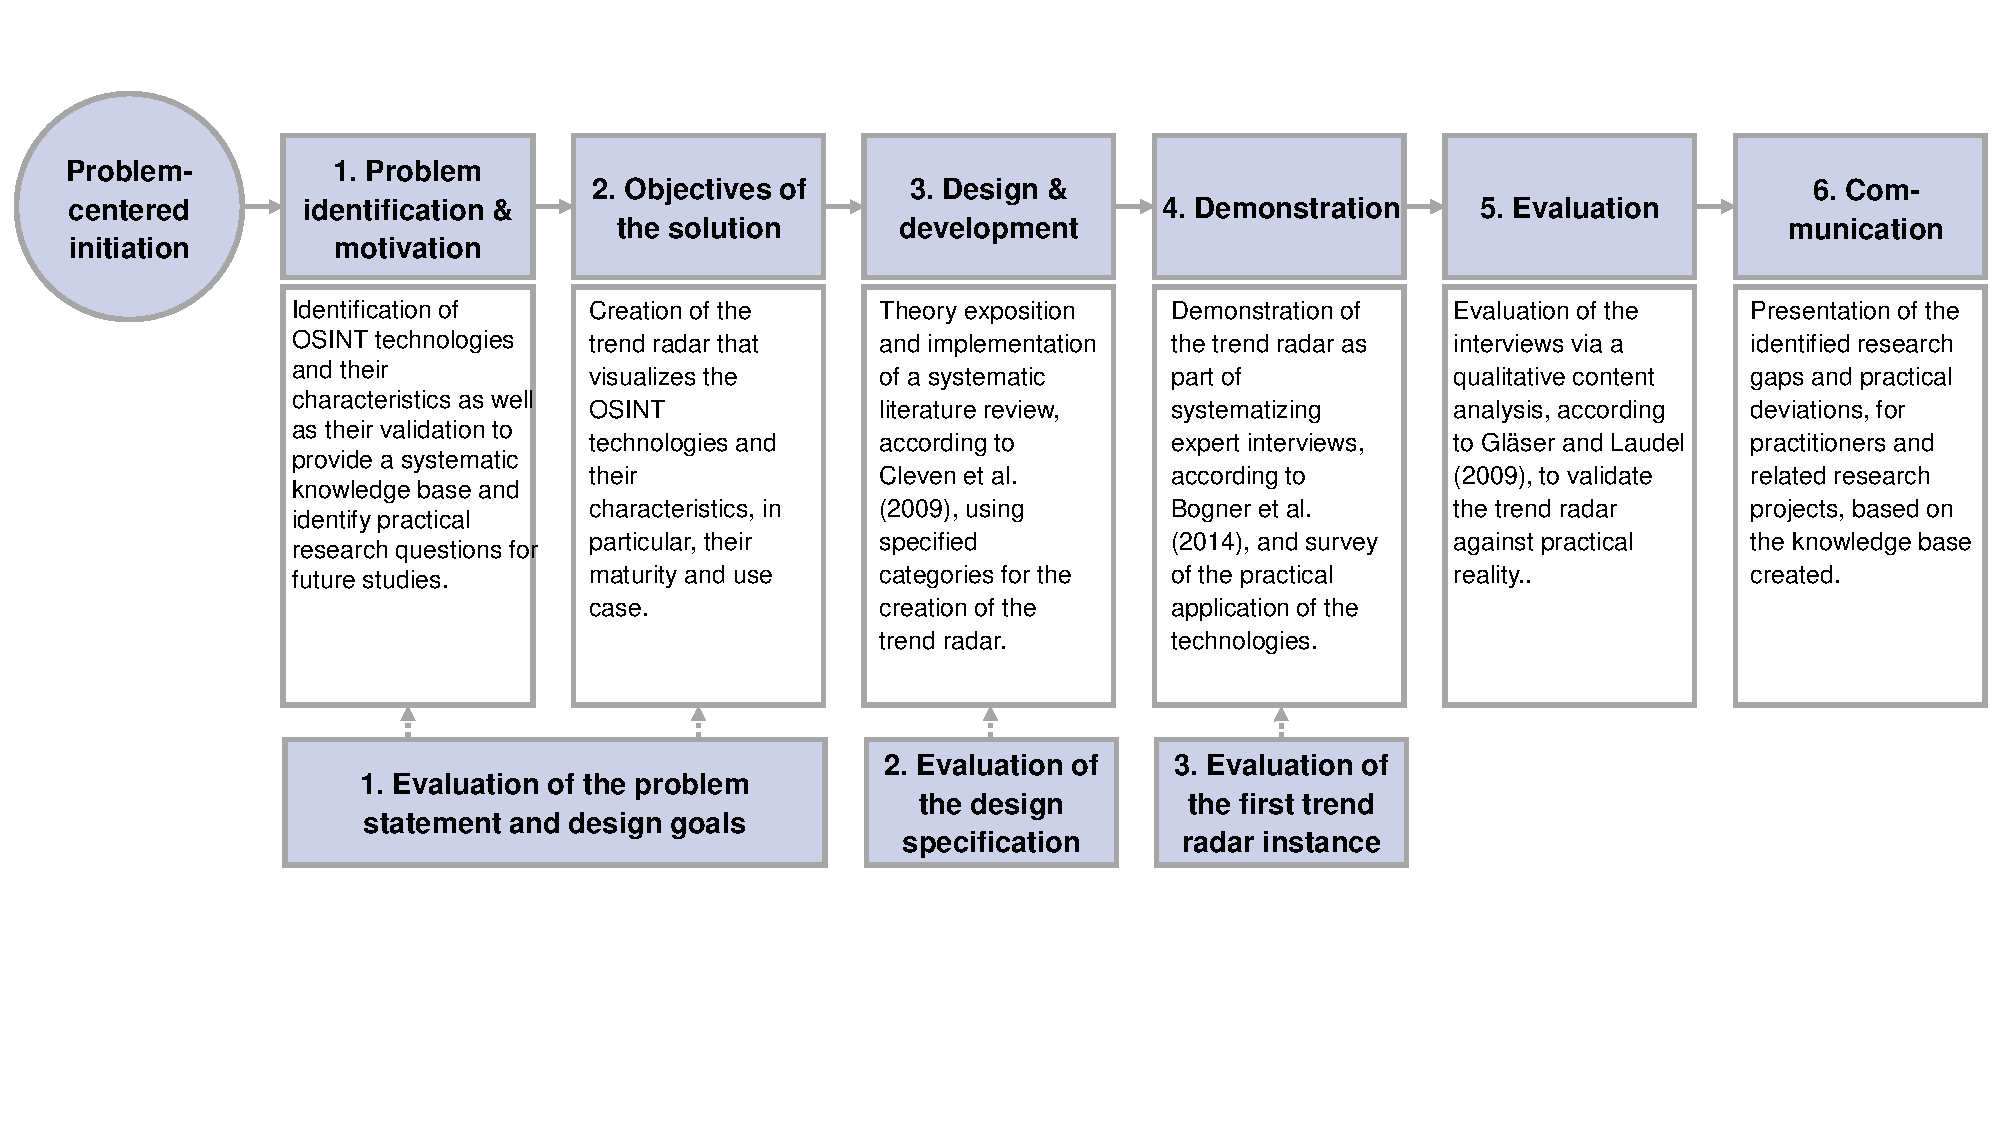
\includegraphics[width=\textwidth]{PDF/images/crop_DSRM}
%    \caption{Design Science Research Model (DSRM)}
%    \label{fig: DSRM}
%\end{figure*}

\subsection{Design Objectives of the Solution} \label{sec:designobjectives}


The design objectives of the solution are divided into content-related objectives (CO) and formal objectives (FO).

\begin{itemize}
    \item[\textbf{CO1}] The trend radar must mirror the intelligence generation process, facilitating structured mapping of identified technologies based on their usage. This enables direct assignment of research gaps to respective phases, verifying the existence of third-generation OSINT systems.
    \item[\textbf{CO2}] Key characteristics, particularly technology maturity levels and use cases, must be considered. Technology maturity informs research status determination, while use cases unveil research directions.
\end{itemize}

\begin{itemize}
    \item[\textbf{FO1}] The trend radar must follow a simple structure for quick identification of research gaps and high standardization for applicability across intelligence disciplines.
    \item[\textbf{FO2}] The trend radar should be continually expandable to capture field dynamics effectively.
\end{itemize}

\subsection{Evaluation of the Problem Statement and Design Objectives} \label{sec:eval}
In Section \ref{sec:theoreticalbackground}, key concepts foundational to the research are defined, focusing on the intelligence cycle. The cycle is crucial as it underpins the development of the trend radar tool, which is evaluated for its compatibility within the OSINT framework. Furthermore, the review of prior studies reveals a significant gap in comprehensive OSINT research, emphasizing the importance and relevance of the inquiry.

\subsection{Design and Development}
The third activity involves conducting a systematic literature review, guided by Cleven et al. \cite{Cleven.2009}. Cooper's taxonomy \cite{Cooper.1988} is used to scope the review, establishing classification categories for creating concept matrices to structure the literature analysis \cite{Webster.2002}.

To standardize the approach across the intelligence cycle, general categories were defined for each phase, integrating the evaluation and feedback phase due to its iterative nature. For the collection phase, six categories were developed:
\begin{itemize}
    \item \textbf{Use case:} Application areas of the technologies.
    \item \textbf{Data:} Composition and types of data foundations, including data format and source.
    \item \textbf{Process:} Degree of automation in the technologies, categorized into manual, semi-automated, automated, and fully automated/autonomous \cite{Duncheon.2002, Billings.1997, Endsley.1999}.
    \item \textbf{Technology:} Material and immaterial means used for managing information \cite{Bleck.2004}.
    \item \textbf{Technology Complexity:} Assessed through subcategories of Volume, Variety, and Velocity \cite{Elgendy.2014, Singh.2012}.
    \item \textbf{Maturity Level:} Based on the phases of innovation, prototype, and market establishment \cite{Stich.2022}.
\end{itemize}

Similar categories were adapted for the other phases of the intelligence cycle, with complexity measured via the analytics spectrum: descriptive, diagnostic, predictive, and prescriptive \cite{Delen.2013}.

The literature search, executed using a broad search string to maximize retrieval, was limited to publications from 2020 to 2023 to reflect recent advancements. A total of 60 studies were analyzed using the SQR3 method \cite{Robinson.1970} and categorized into a meticulously structured Excel spreadsheet for each phase of the intelligence cycle (Fig. \ref{fig:LiteratureReview}).

\begin{figure}[t]
    \centering
    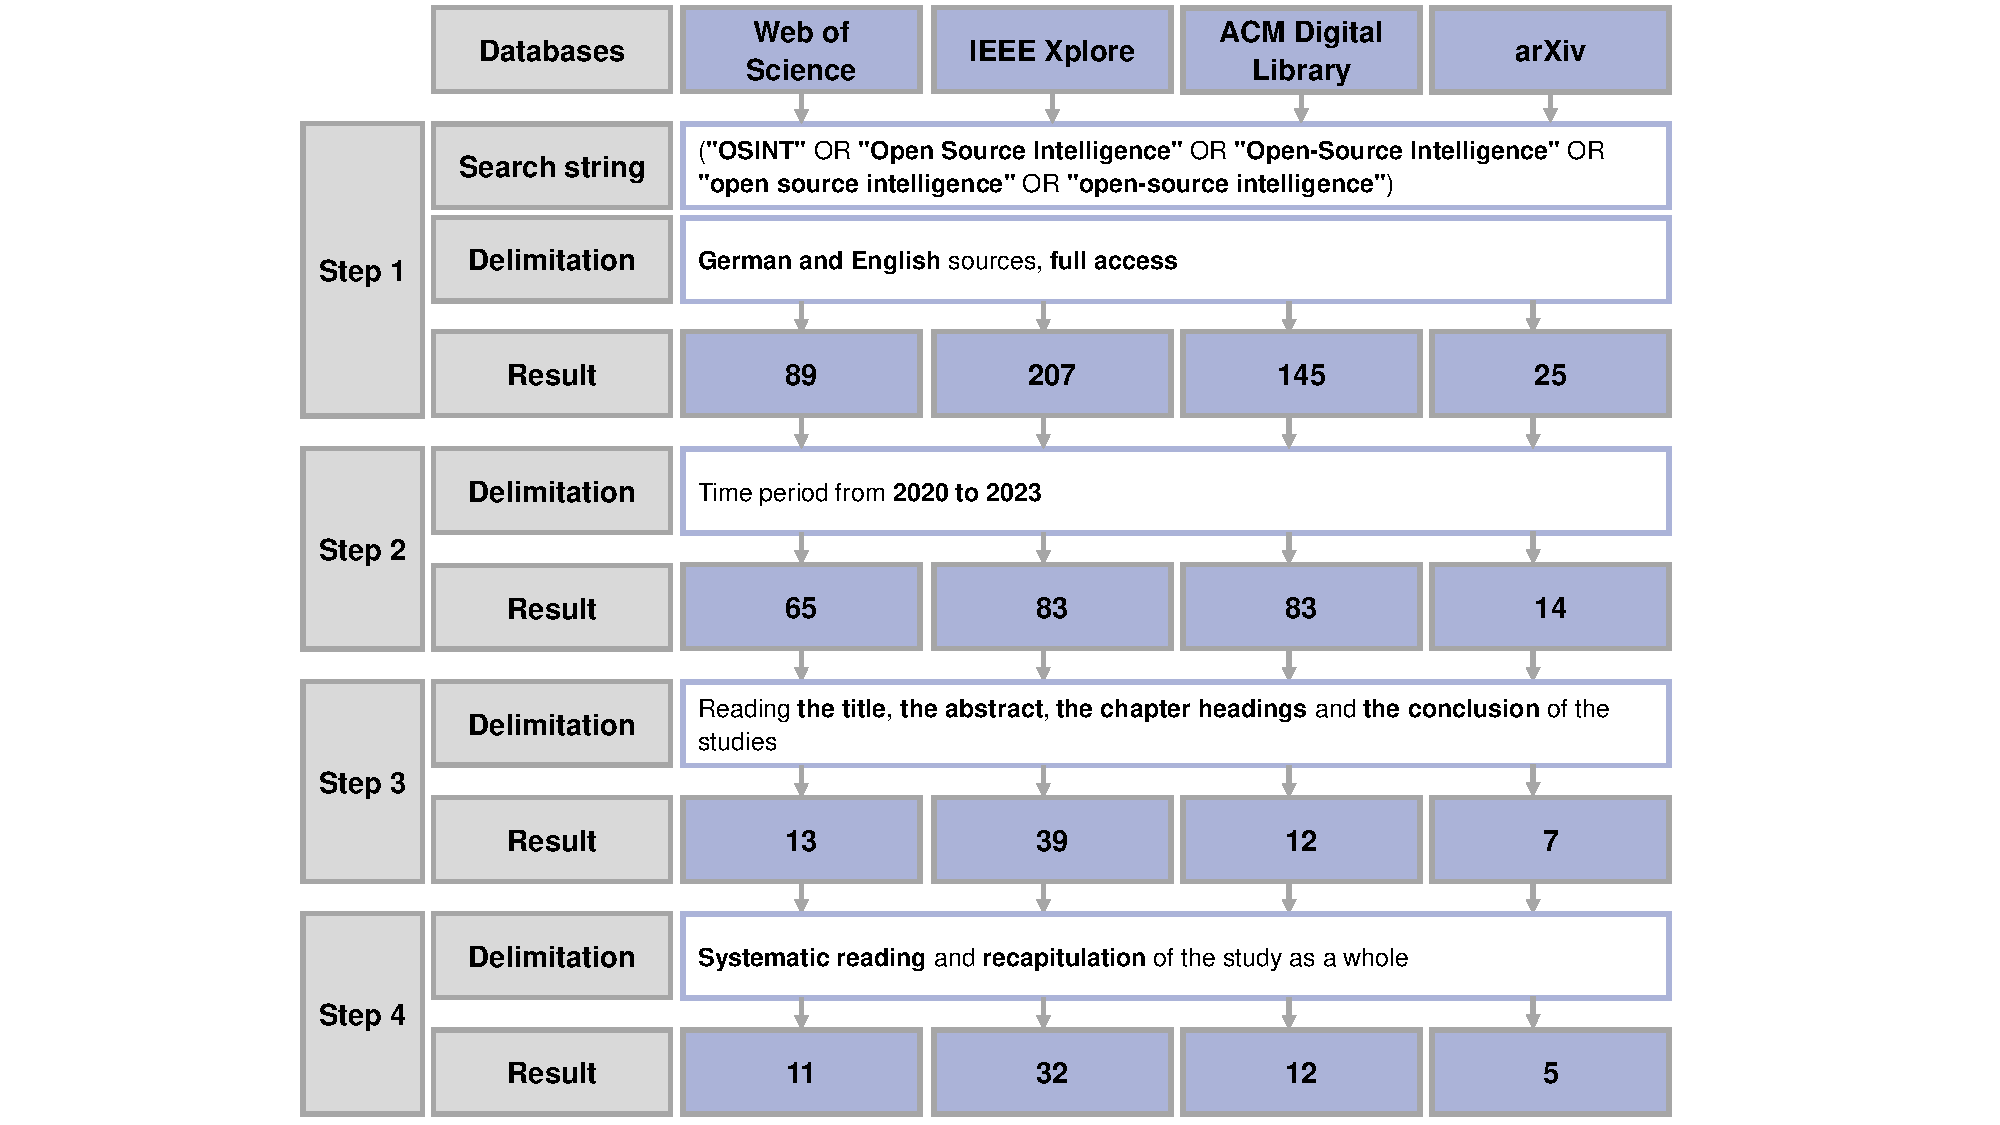
\includegraphics[width=0.4\textwidth]{PDF/images/crop_Kategorisierungskriterien und Literraturreviewaufbau}
    \caption{Literature review setup and categorization criteria}
    \label{fig:LiteratureReview}
\end{figure}

Each technology was then categorized and analyzed for interrelationships within the OSINT framework. Verification of categorization was conducted using a Python script, which scanned the included papers for predefined keywords. The validated categories and relationships informed the development of the trend radar based on the verified concept matrices.


\subsection{Evaluation of the Design Specifications}
The intelligence cycle forms the foundation of the trend radar, offering clarity and an intuitive framework that simplifies technology extraction and research gap identification. Its design also ensures applicability across diverse intelligence disciplines. By emulating the structure of the federal government's trend radar \cite{Stich.2022}, it achieves robustness, user-friendliness, and appropriate detail, focusing on essential categories like use case, technology, and maturity level.

The concept matrices enable regular updates to the radar, ensuring current and standardized design. Rigorous verification of internal consistency maintains categorization integrity, meeting critical evaluation criteria in contemporary design research \cite{vomBrocke.2020b}.


\subsection{Demonstration}
Next, the trend radar was demonstrated via guideline-based, systematizing expert interviews \cite{Bogner.2014, Glaser.2009, Meuser.1991}. Particularly in less structured and sparsely linked subject areas, this method enables dense data collection \cite{Bogner.2014, Meuser.1991}, especially when access to the social field is limited \cite{Bogner.2002c, Glaser.2009}.

Experts (table \ref{tab:experts}) were selected using theoretical sampling \cite{Glaser.1967}, focusing on Germany to validate trends in the country. At least one expert from a security authority, the security industry, and a startup was chosen to capture diverse perspectives. A "prestigious" company position ensures respondents possess relevant research knowledge \cite{Bogner.2002b}.

\begin{table}[htbp]
    \caption{Interviewed experts}
    \begin{tabular}{p{0.25\linewidth}p{0.55\linewidth}p{0.05\linewidth}}
        \toprule
        \textbf{Organization} & \textbf{Position}                                             & \textbf{ID} \\
        \hline
        Industry/ Authority   & Senior Intelligence Consultant                                & E1          \\
        \hline
        Industry/ Authority   & Referent Corporate Security                                   & E2          \\
        \hline
        Authority             & In-House Senior Consultant                                    & E3          \\
        \hline
        Start-up              & Managing Director of a German start-up, for an OSINT platform & E4          \\
        \bottomrule
    \end{tabular}
    \label{tab:experts}
\end{table}
The qualitative data collection utilized semi-structured interviews, ideal for uncovering underlying theoretical relationships \cite{Bogner.2014}. The questionnaire, based on the Intelligence Cycle, commenced with a presentation of the trend radar. Open questions were initially posed for each phase to compare it with respondents' practical experience, reducing subjectivity \cite{Saunders.2012}. Exploratory questions guided conversation flow \cite{Saunders.2012}, followed by specific closed questions for targeted follow-up \cite{Saunders.2012}. The Interviews lasted up to an hour, with a maximum of three main questions per phase \cite{Bogner.2014} and were conducted online. The questionnaire underwent pilot testing with a domain expert.

\subsection{Evaluation of the First Instance of the Trend Radar}

The trend radar demonstration affirmed its intuitive usability and usefulness in providing an overview of OSINT technologies. Practitioners also confirmed its completeness and internal consistency (cf. E1, 14.08.2023; E3, 28.07.2023; E4, 02.08.2023). As a result, the radar proved suitable for identifying research gaps and guiding practitioners. Thus, it meets the essential evaluation criteria \cite{Sonnenberg.2012}.

\subsection{Evaluation}

The evaluation utilized qualitative data analysis \cite{Glaser.2009}, which extracts, synthesizes, and structures interview information using a predefined search grid. This facilitates targeted extraction and summarization of relevant, cross-interview information, following a "top-down approach" \cite{Bogner.2014, Glaser.2009}.

First, the interviews were transcribed, followed by analysis using the MAXQDA software. The categorization grid was established within MAXQDA (see repository X), with first-level categories corresponding to the phases of the intelligence cycle. Second-level categories indicate support or contradiction of the experts to the theory, while third-level categories reflect identified use cases. A "general statements" category was thereby added for overarching remarks. The fourth-level categories classify the individual technologies. In total, 257 statements were categorized.

\section{Results} \label{sec:results}

The trend radar (figure \ref{fig:trendradar}, \ref{fig:trendradarexplanation}) is read from the outermost to the innermost.
Each fifth of the cycle represents an Intelligence Cycle phase. Subdivisions indicate
phase-specific use cases, while color gradations show maturity levels. Numbered black
and white dots denote grouped technologies, presented in a boxplot-like format reflecting
varying maturity levels.

\begin{figure*}[thb]
    \centering
    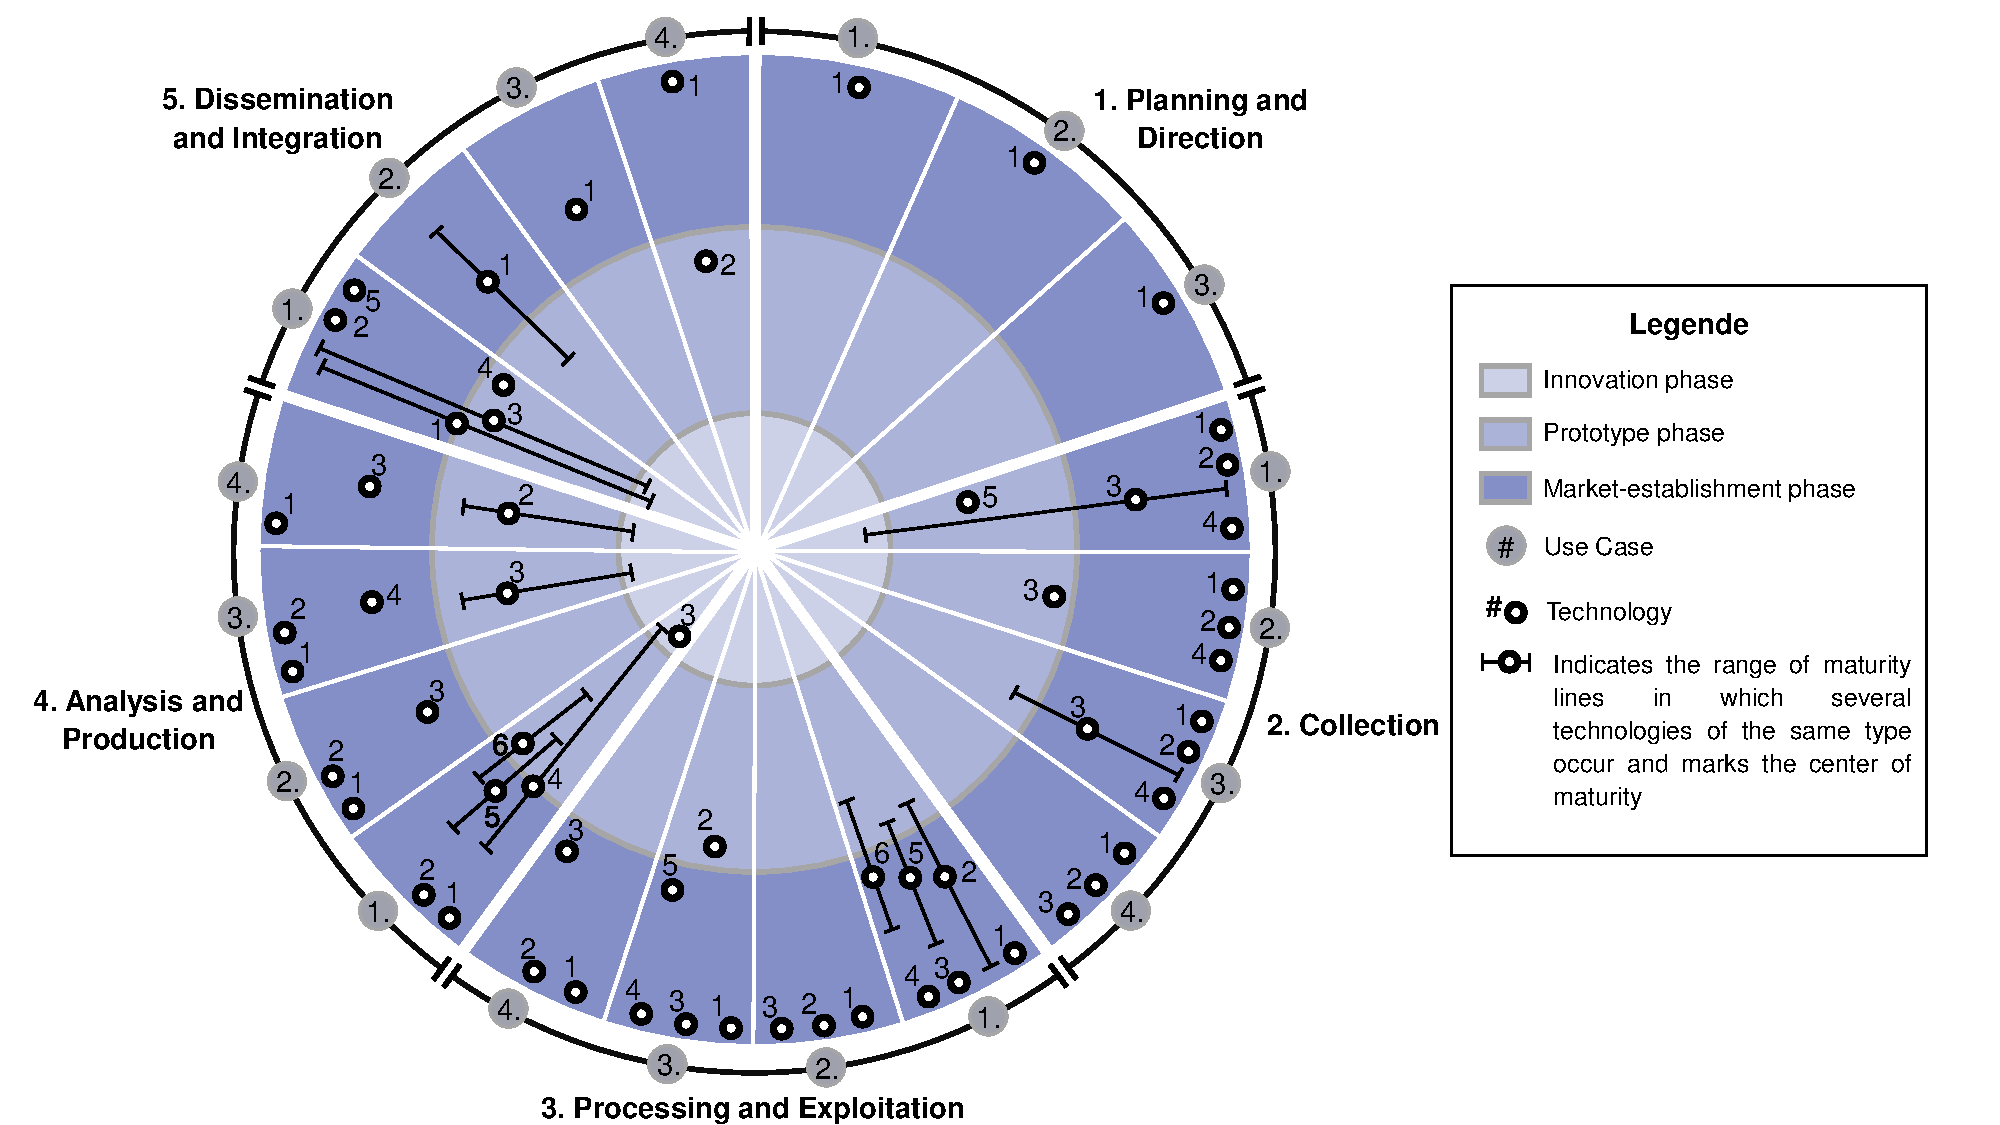
\includegraphics[width=0.8\textwidth]{PDF/images/crop_Trendradar}
    \caption{Trend radar}
    \label{fig:trendradar}
\end{figure*}

\begin{figure*}[thb]
    \centering
    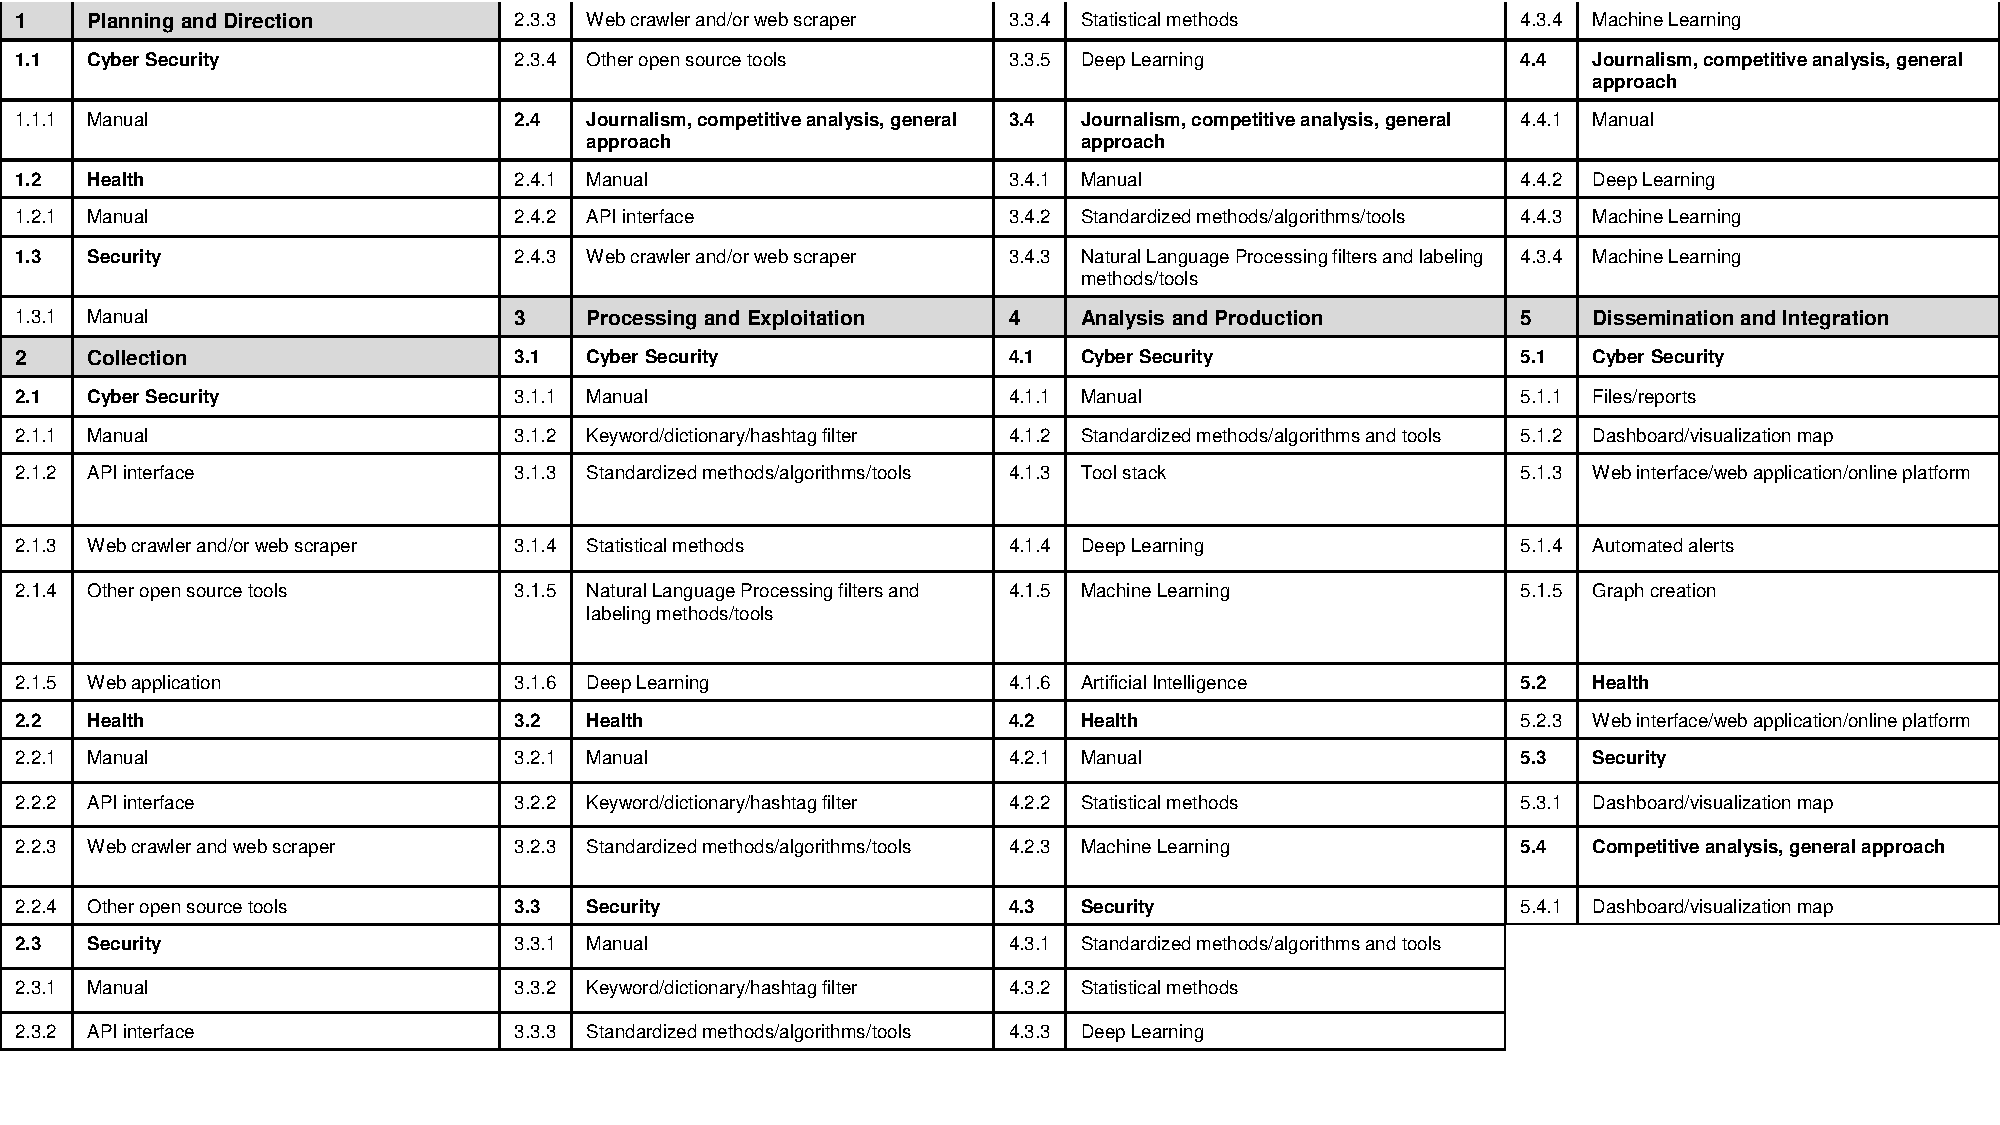
\includegraphics[width=0.99\textwidth]{PDF/images/crop_Trendradar explanation}
    \caption{Trend radar explanation}
    \label{fig:trendradarexplanation}
\end{figure*}

\subsection{Intelligence Cycle in Theory-Practice Comparison}

Studies align with each phase of the Intelligence Cycle, but no application covers all phases as a third-generation OSINT tool. Literature mainly focuses on the collection phase, followed by analysis and production, and processing and exploitation. The dissemination and integration phase is least covered, followed closely by planning and direction.

These findings align with the experts' practical experiences. They regard the Intelligence Cycle as "state of the art" (cf. E3, 28.12.2023), but note different manifestations of the phases in praxis (cf. E4, 02.08.2023).
The planning and direction phase is often neglected, despite its crucial importance, leading to wasteful production (cf. E3, 28.07.2023). Conversely, OSINT is frequently associated solely with the collection phase,
resulting in subpar outcomes due to high volumes of low-quality data (cf. E1, 14.07.2023; E2, 19.07.2023; E3, 28.07.2023). The main reason for this is, that the Intelligence Cycle is operated by at least three groups of people. Firstly, the customers, usually located at the "decision-maker level", with a primarily legal professional background (cf. E2, 19.07.2023).
The second is the technician who carries out the data collection and processing (cf. E2, 19.07.2023; E3, 28.07.2023). Lastly, the analyst evaluates the data and creates the intelligence product (cf. E1, 14.07.2023). The process thereby is rarely transparent between the parties
(cf. E1, 14.07.2023; E2, 19.07.2023) and is rarely anchored at the organizational level (cf. E4, 02.08.2023). According to the experts, there is thus no third-generation
OSINT tool in use, at least not in German authorities. In addition, the collection focus is driven by concerns about missing vital information, which could later be revealed as publicly available (cf. E1, 14.07.2023).

\subsection{Use Cases in Theory-Practice Comparison}

Five main use cases emerged from the research: Cyber Security, Health, Security, Journalism,
and Competition Analysis. Cyber Security studies primarily focus on Open Source Cyber Threat
Intelligence (OSCTI), which involves collecting, monitoring, and analyzing public
data to detect potential cyber threats \cite{Ahuja.2022,AlDmour.2023}.
Health applications mainly address COVID-19 outbreak investigations \cite{Kpozehouen.2020}.
The security use case includes applications such as
analyzing violent behavior in public transport \cite{Nobili.2021}. The identified journalism study examines the
Twitter activities of the OSINT journalists' association "Bellingcat" \cite{Bar.2023}. Competitive analysis
involves for example the performance classification of Chinese logistics companies \cite{Tao.2023}.
Additionally, two identified studies focus generally on creating knowledge graphs on OSINF \cite{Hu.2023, Ma.2022}.

The Experts indicate that OSINT is used in all authorities and various use cases, even if not explicitly labeled as such (cf. E2, 19.07.2023). It is most commonly applied in cybersecurity/CTI (cf. E1, 14.07.2023; E2, 19.07.2023) and general security, especially within the German Armed Forces, the (Federal) Intelligence Service, domestic intelligence services, and the police.

\subsection{Technologies and Maturity Levels in Theory-Practice Comparison}

Except for the initial phase, automated technologies are utilized across all subsequent phases and use cases.
These technologies demonstrate considerable market maturity, yet manual activities remain prevalent.
The highest level of automation is observed in the CTI use case.

The most advanced automated technologies in the collection phase are web crawlers and/or web scrapers.
Established technologies include "off the shelf" tools (cf. \cite{Middleton.2020}) and open source
solutions like "Tweepy", a Python library for Twitter crawlers (e.g., \cite{Adewopo.2020}).
More advanced prototypes involve combining parallelized, recursive, source-specific web crawlers and scrapers for improved
data collection (e.g., \cite{Jenkins.2021}). Another method in the prototype phase is
"focused crawling", adapting the crawling path dynamically using a content-driven ML algorithm, BERT ("Bidirectional Encoder Representation from Transformers")
\cite{Kuehn.2023}. Technologies for crawling/scraping the dark web, like "Torsion" \cite{Sonawane.2022},
were assigned to the innovation phase. The experts also note the increasing use of open source tools alongside manual work
(cf. E1, 14.07.2023; E3, 28.07.2023; E1, 14.07.2023). However, they consider traditional web crawling and scraping
outdated due to errors, implementation difficulties, and website resistance. Screenshot-based "web shooting" with
OCR (Optical Character Recognition) extraction is seen as more modern and robust (cf. E3, 28.07.2023).

NLP applications/methods such as "Topic Classifying", "Part-of-Speech Tagging", "Entity and Relation Annotation", and "Named Entity Recognition"
demonstrate high automation levels in the processing and utilization phase. Technologies commonly used include
the "Python NLTK Toolkit" \cite{Hubbard.2022} and the "Stanford CoreNLP Toolkit" \cite{Middleton.2020}.
Additionally, deep learning, particularly through "word embedding" using the "word2vec" algorithm, is prominent
(e.g., \cite{Bai.2020}).


However, the experts note that within authorities this phase predominantly involves manual work due to irreplaceable domain knowledge
(cf. E1, 14.07.2023; E2, 19.07.2023; E3, 28.07.2023). The degree of automation depends on the abstraction level:
operational tasks needing specific information show lower automation than long-term strategic analyses requiring
extensive data (cf. E3, 28.07.2023).

The highest automation level is observed in the analysis and production phase, where AI, ML, and DL technologies are prevalent.
Under DL, vectorization algorithms can also be found. Particularly BERT algorithms in different versions are commonly utilized
(e.g., \cite{Ma.2022}). Furthermore, even under ML vectorization models such as BERT or
"Supervised Support Vector Machines" (SVM) (e.g., \cite{Iorga.2020}) are listed.
In addition, the algorithms "Random Forest", XGBoost ("eXtreme Gradient Boosting)",
lightGBM ("light Gradient Boosting Machine"), "Naive Bayes" and "logistic regressions" are particularly common.
Publications thereby often utilize multiple algorithms concurrently for performance comparison (e.g., \cite{Tao.2023})
or for layered analysis (e.g, \cite{Yang.2022}). AI technologies are less specified,
except for Dale et al. \cite{Dale.2023}, who developed a bidirectional recurrent neural network with
BiGur ("Bidirectional Gated Recurrent Unit") layers. Due to the modular use of publicly available models,
the technologies are mostly classified as market-ready. The experts note, that this phase largely relies
on manual content analysis due to limited technological understanding and acceptance, in german authorities
(cf. E2, 19.07.2023; E3, 28.07.2023; E4, 02.08.2023). Also, ethical and legal barriers, like GDPR (General Data Protection Regulation), hinder technology
adoption (cf. E2, 19.07.2023; E4, 02.08.2023). Additionally, security concerns favor standalone systems,
with smart technologies often used unofficially (cf. E2, 19.07.2023; E4, 02.08.2023). However, there is a need for modular,
expandable systems to keep pace with advancements (cf. E1, 14.07.2023; E3, 28.07.2023; E4, 02.08.2023). Nevertheless, human experience
and specialization remain crucial to ensure product quality. Yet, the potential of Large Language Models (LLM) remains uncertain (cf. E4, 02.08.2023).

In the dissemination and integration phase, tools like "Power BI" \cite{Tao.2023}
are utilized to create dashboards and visualization maps. Furthermore, user interfaces,
web applications, and online platforms are developed, including Python GUIs,
specific browser applications \cite{Elmas.2022},
improved user interfaces and input masks for entire tool stacks \cite{Arjun.2020}.
Additionally, automated alert technologies for cybersecurity risk assessments are prevalent \cite{Ahuja.2022}. Graph-based visualizations are also common, utilizing tools
/libraries like "Matplot," "Networkx," "Pygraphistry," or the "Neo4j-Browser" \cite{Middleton.2020}.
Except from the alerts, the retrieval of results is largely semi-automated, with technologies in the market establishment phase. No information on targeted user tests or new development runs involving user feedback was found in any of the studies. The experts state that there is still very little
automation within the authorities during this phase. The final product often comprises only a PDF document, email, or verbal report (cf. E1, 14.07.2023), which suffices in many cases (cf. E3, 28.07.2023).
However, beyond OSINT, various automated tools exist that could be applied to the authorities (cf. E4, 02.08.2023). Moreover, there is a lack of necessary feedback for product improvement in practice (cf. E3, 28.07.2023).

\section{Discussion and Conclusion} \label{sec:discussion}
%\section{Discussion} \label{sec:discussion}
\subsection{Contributions and Implications}

The investigation into the existence of a robust, automated third-generation OSINT system (e.g., \cite{Ghioni.2023}) concludes negatively for Germany. Identified applications do not fully cover the intelligence cycle, particularly lacking in the planning and direction phase, followed by dissemination and integration. Hence, human analysis remains crucial. However, the finding by Pastor-Galindo et al. \cite{PastorGalindo.2020} that intelligent OSINT
concepts are not yet widespread cannot be confirmed either. Numerous intelligent tools available
on the market were identified in the other phases. Nevertheless, practical integration has so far
fallen short of the (theoretical) possibilities. Yet this finding likewise does not confirm the
thesis of Yogish et al. \cite{Yogish.2021} that automated, AI-driven solutions, largely eliminating
the human component, are indispensable in all OSINT domains. The key research
question should be why proven, available applications whose support is needed have not
yet found widespread use, especially in german intelligence authorities. Additionally, research should explore how to enhance technical support for the initial and final phases of the Intelligence Cycle

Addressing these research questions entails resolving numerous underlying research gaps (RGs), directly corresponding to the three key groups involved in the intelligence cycle.

%\begin{itemize}
%    \item[\textbf{RG1:}] \textbf{Deficiency in Initial Phase Tools:} There is a technological gap in tools that cover the initial phase of the intelligence cycle, particularly in frameworks for targeted requirements definition and communication. This gap contributes to an overemphasis on the collection phase \cite{Lowenthal.2020}.
%
%    \item[\textbf{RG2:}] \textbf{Lack of Dissemination Mechanisms:} There is a dearth of effective dissemination and integration mechanisms tailored for authorities, largely due to insufficient user testing and iterative feedback incorporation. The indispensability of consumer feedback is underscored by established frameworks to enhance product quality and reduce data overload \cite{DirectorofNationalIntelligence.2011,JointChiefsofStaffU.S.Army.2013,NorthAtlanticTreatyOrganization.2001,Gibson.2016,Day.2016}.
%
%    \item[\textbf{RG3:}] \textbf{Modular OSINT Systems:} The future of OSINT systems hinges on modular concepts, yet only limited research has been conducted in this area \cite{Arjun.2020,Wright.2020}.
%
%    \item[\textbf{RG4:}] \textbf{Revamping Procurement Procedures:} It's crucial to move away from monolithic stand-alone setups in procurement procedures.
%
%    \item[\textbf{RG5:}] \textbf{Ethical and Legal Compliance:} Ensuring compliance with ethical and legal principles is vital for product adoption, requiring robust legislative updates and considering both national and international regulations, such as GDPR \cite{EuropeanParliament.2016,EuropeanCommission.18.08.2023,Ghioni.2023,Wittmer.2022}.
%
%    \item[\textbf{RG6:}] \textbf{Technical Understanding among Decision Makers:} Addressing challenges necessitates foundational technical understanding at decision-maker levels, fostering openness to technology and cultivating an information-sharing mindset to transcend bureaucratic barriers \cite{NorthAtlanticTreatyOrganization.2001}.
%
%    \item[\textbf{RG7:}] \textbf{Use of LLMs in Intelligence:} While Large Language Models (LLMs) show promise in intelligence analysis, their application in operational settings is underexplored \cite{Radford.2023,Zhao.31.03.2023}.
%
%    \item[\textbf{RG8:}] \textbf{Technological Tools for Technicians:} Technicians often handle significant phases of the intelligence cycle independently, yet there is a notable absence of robust collection tools to match the rapidly evolving media landscape.
%
%    \item[\textbf{RG9:}] \textbf{Coordination between Analysts and Technicians:} Coordination gaps between analysts and technicians pose risks of excessive data collection, emphasizing the need for tools that enhance transparency and mitigate collection biases \cite{Lowenthal.2020}.
%\end{itemize}

\begin{itemize} 
    \item[\textbf{RG1:}] There is a technological gap in tools that cover the initial phase of the intelligence cycle, particularly in frameworks for targeted requirements definition and communication.
%This gap contributes to an overemphasis on the collection phase \cite{Lowenthal.2020}.

\item[\textbf{RG2:}]Effective dissemination and integration mechanisms tailored for authorities are deficient, primarily due to inadequate user testing and iterative feedback incorporation. The importance of consumer feedback is underscored by established frameworks to enhance product quality and mitigate data overload \cite{JointChiefsofStaffU.S.Army.2013, NorthAtlanticTreatyOrganization.2001}.

\item[\textbf{RG3:}] The future of OSINT systems hinges on modular concepts, yet only limited research has been conducted in this area \cite{Arjun.2020,Wright.2020}.

\item[\textbf{RG4:}] It's crucial to move away from monolithic stand-alone setups in procurement procedures.

\item[\textbf{RG5:}] Ensuring compliance with ethical and legal principles is vital for product adoption, requiring robust legislative updates and considering both national and international regulations, such as GDPR \cite{EuropeanParliament.2016,EuropeanCommission.18.08.2023,Wittmer.2022}.

\item[\textbf{RG6:}] Addressing challenges necessitates foundational technical understanding at decision-maker levels, fostering openness to technology and cultivating an information-sharing mindset to transcend bureaucratic barriers \cite{NorthAtlanticTreatyOrganization.2001}.

\item[\textbf{RG7:}] While LLMs show promise in intelligence analysis, their operational application remains underexplored \cite{Radford.2023,Zhao.31.03.2023}.

\item[\textbf{RG8:}] Technicians often handle significant phases of the intelligence cycle independently, yet there is a notable absence of robust collection tools to match the rapidly evolving media landscape.

\item[\textbf{RG9:}] Coordination gaps between analysts and technicians pose risks of excessive data collection, emphasizing the need for tools that enhance transparency and mitigate collection biases \cite{Lowenthal.2020}.
\end{itemize}
%These gaps highlight the critical areas for future development and research to enhance the efficiency and effectiveness of intelligence operations.

\subsection{Limitations and Future Research}

The first limitation relates to the fact that, due to a lack of clarity about the legal
and ethical basis \cite{Ghioni.2023,Wittmer.2022},
it could not be verified whether only public sources \cite{NorthAtlanticTreatyOrganization.2002} were used
in the analyzed studies. It was also not verified whether the technologies meet the
legal and ethical requirements for the use of the information obtained
\cite{PastorGalindo.2020,Wittmer.2022}. The second
limitation stems from classification categories not fully aligning with the
MECE (Mutually-Exclusive-and-Collectively-Exhaustive) principle \cite{Lee.2018},
particularly evident in the hierarchical dependency of AI, ML, and DL technologies. In addition,
the wording of the authors was followed for objective reproduction when identifying the technologies,
but the accuracy of the information was not reviewed in detail. Moreover, no fixed limits could be defined
for the volume category, as these were not recorded in uniform dimensions in the studies.
The third limitation concerns the limited sample size in expert interviews. Due to the
extremely difficult-to-access target group, interviews were not conducted with active users and decision-makers within authorities.
Also, independent verification of coding by a second researcher is recommended for improved intercoder reliability 
\cite{Bogner.2002c, Glaser.2009}. Lastly, the research structure followed a linear execution rather than the suggested iterative approach \cite{Peffers.2007}.

Nevertheless, the study furnishes future researchers with a comprehensive knowledge base on OSINT
through a practice-validated trend radar.
%The radar serves as a comprehensive knowledge base, allowing for contemporary evaluation and analysis of OSINT technologies.
Initial evaluations reveal two crucial unanswered research questions and identifies nine detailed research gaps, highlighting
critical areas for future development and research to enhance the efficiency and effectiveness of intelligence operations.
%as well as identifying research gaps for future studies, penetrating the complex research field. 
Moreover, the developed trend radar serves as a guideline for practitioners. The radar
is adaptable to the evolving subject area and transferable to other intelligence disciplines.


%Before addressing these questions, future researchers are advised to validate them further. 
%Utilizing the presented tools to reevaluate literature
%categorization and update identified technologies is recommended. In addition, semantic
%control and indexing methods (e.g. LLM) should be included. Due to the high dynamic of the research field,
%it is also recommended to integrate news articles and scientific journals with shorter publication cycles.
%Reassessing categories based on MECE criteria and conducting further interviews, including internationally
%and with active authority members, is advisable. Employing methods like the Delphi technique to evaluate
%trends and establish consensus is suggested \cite{Hader.2000}. Subsequent iterations of the design process and adjustments
%to the trend radar, if necessary, should follow based on these results \cite{Peffers.2007,Sonnenberg.2012}.

%\subsection{Conclusion}
%\subsection{Summary}

%In this paper, a practice-validated trend radar was developed that depicts current trends
%in the field of OSINT through applied technologies. It serves as a comprehensive knowledge base,
%allowing for contemporary evaluation and analysis of OSINT technologies as well as identifying research
%gaps for future studies, penetrating the complex research field. Moreover, it serves as a guideline for practitioners. The radar
%is adaptable to the evolving subject area and transferable to other intelligence disciplines.
%Based on the developed trend radar, current research gaps are identified and new research questions are raised.

%Results reveal the absence of an automated third-generation OSINT system in Germany, highlighting the
%need for technological support in the planning and direction as well as the dissemination and integration phases.
%The research questions identified for future studies are therefore, why proven, available applications,
%have not yet found widespread use, especially in the security authorities.
%In addition, the question of how the first and last Intelligent Cycle phases, alongside the others,
%can be better supported technically is to be investigated. The research gaps identified extend
%not only to technology but in particular to the legal, administrative, political and
%social sciences, necessitating interdisciplinary collaboration. Above all, a need to catch up is seen
%in the non-technical research fields, responsible for creating the decisive prerequisites for technology
%implementation.


% Fonts specification --- not shown as it doesn't exist in the Word document either. 

%\section{Fonts}

%A summary of fonts is provided in Table \ref{tab: fonts}. 

%\begin{table}[thb]
%\centering
%\caption{\label{font-table} Font guide. \vskip 3pt }
%\label{tab: fonts}
%\begin{tabular}{l|rl}
%\hline \bf Type of Text & \bf Font Size & \bf Style \\ \hline
%paper title & 14 pt &  \bf bold \\
%authors & 10 pt &  \underline{email} underlined \\
%abstract title & 12 pt &  \bf bold\\
%abstract text & 10 pt &  \it italic\\
%section titles & 12 pt & \bf bold \\
%subsection titles & 11 pt & \bf bold \\
%document text & 10 pt  & \\
%captions & 9 pt & \sansserifformat{\captionsize sans-serif, \bf bold} \\
%bibliography & 9 pt & \\
%footnotes & 8 pt & \\
%\hline
%\end{tabular}
%\end{table}


\section{References}


%Bibliography 

\bibliographystyle{ieeetr}
\bibliography{references}

\end{document}
